\documentclass{standalone}
\usepackage{tikz}
\usetikzlibrary{patterns, positioning}

\begin{document}
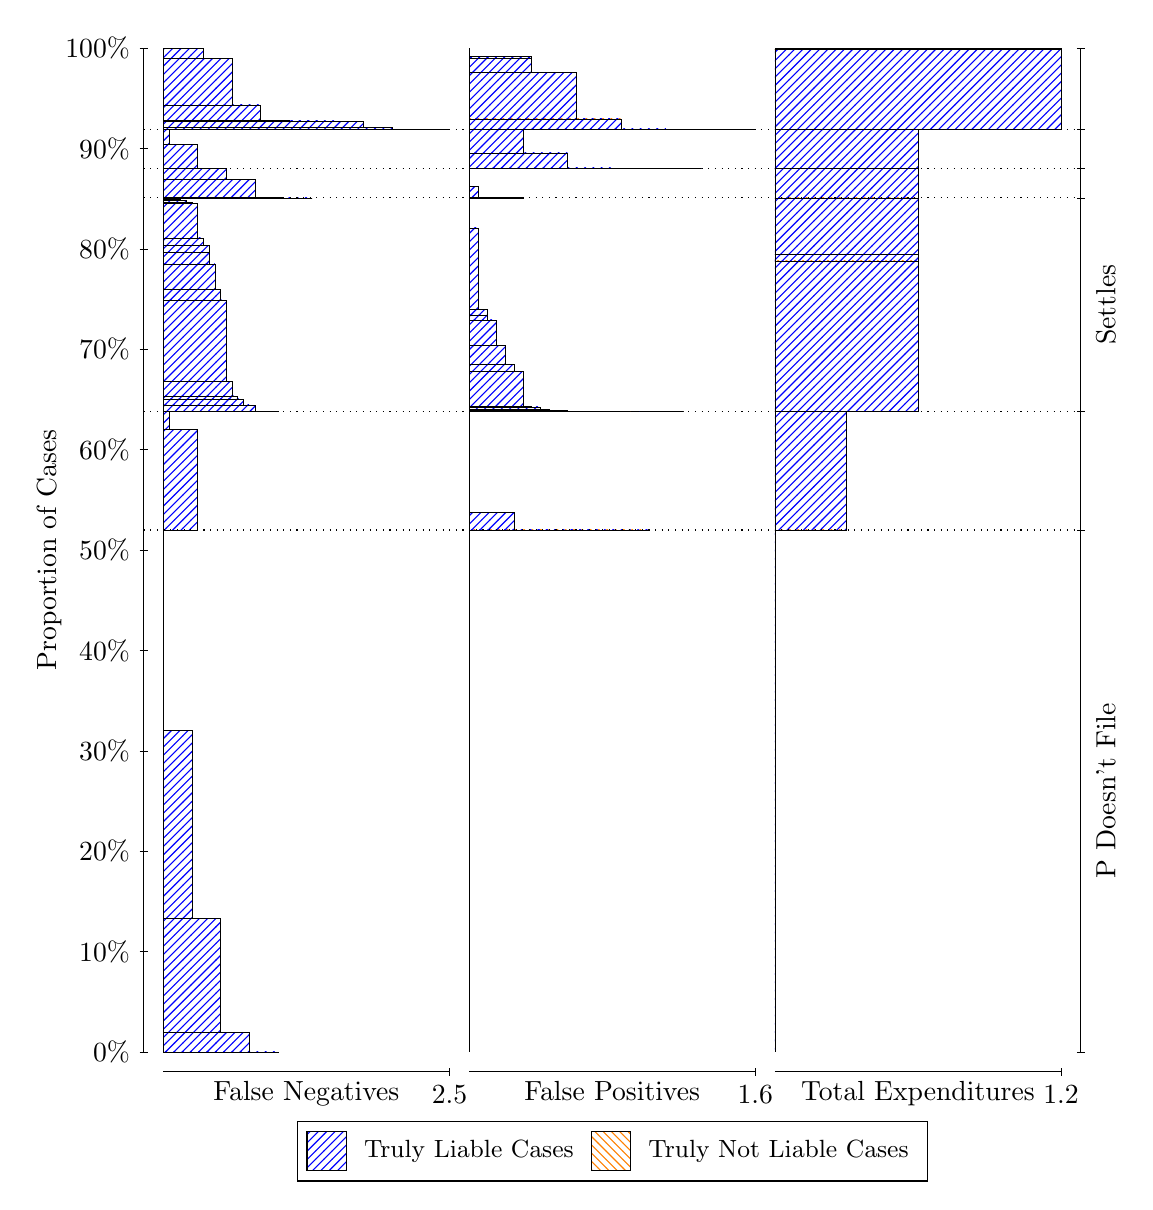
\begin{tikzpicture}
\draw[black, very thin] (1.5,1.75) -- (1.5,14.5);
\node[rotate=90, anchor=center] at (0.3, 8.125) {Proportion of Cases};
\draw[black, very thin] (1.45,1.75) -- (1.55,1.75);
\node[anchor=east] at (1.45, 1.75) {0\%};
\draw[black, very thin] (1.45,3.025) -- (1.55,3.025);
\node[anchor=east] at (1.45, 3.025) {10\%};
\draw[black, very thin] (1.45,4.3) -- (1.55,4.3);
\node[anchor=east] at (1.45, 4.3) {20\%};
\draw[black, very thin] (1.45,5.575) -- (1.55,5.575);
\node[anchor=east] at (1.45, 5.575) {30\%};
\draw[black, very thin] (1.45,6.85) -- (1.55,6.85);
\node[anchor=east] at (1.45, 6.85) {40\%};
\draw[black, very thin] (1.45,8.125) -- (1.55,8.125);
\node[anchor=east] at (1.45, 8.125) {50\%};
\draw[black, very thin] (1.45,9.4) -- (1.55,9.4);
\node[anchor=east] at (1.45, 9.4) {60\%};
\draw[black, very thin] (1.45,10.675) -- (1.55,10.675);
\node[anchor=east] at (1.45, 10.675) {70\%};
\draw[black, very thin] (1.45,11.95) -- (1.55,11.95);
\node[anchor=east] at (1.45, 11.95) {80\%};
\draw[black, very thin] (1.45,13.225) -- (1.55,13.225);
\node[anchor=east] at (1.45, 13.225) {90\%};
\draw[black, very thin] (1.45,14.5) -- (1.55,14.5);
\node[anchor=east] at (1.45, 14.5) {100\%};

\draw[black, very thin] (13.4,1.75) -- (13.4,14.5);
\draw[black, very thin] (13.35,1.75) -- (13.45,1.75);
\node[anchor=west] at (13.35, 1.75) {};
\draw[black, very thin] (13.35,8.3794) -- (13.45,8.3794);
\node[anchor=west] at (13.35, 8.3794) {};
\draw[black, very thin] (13.35,9.884) -- (13.45,9.884);
\node[anchor=west] at (13.35, 9.884) {};
\draw[black, very thin] (13.35,12.597) -- (13.45,12.597);
\node[anchor=west] at (13.35, 12.597) {};
\draw[black, very thin] (13.35,12.971) -- (13.45,12.971);
\node[anchor=west] at (13.35, 12.971) {};
\draw[black, very thin] (13.35,13.469) -- (13.45,13.469);
\node[anchor=west] at (13.35, 13.469) {};
\draw[black, very thin] (13.35,14.5) -- (13.45,14.5);
\node[anchor=west] at (13.35, 14.5) {};

\draw[black, very thin, pattern color=blue, pattern=north east lines] (1.75,1.75) rectangle (3.2033,1.7525);
\draw[black, very thin, pattern color=blue, pattern=north east lines] (1.75,1.7525) rectangle (2.84,1.9968);
\draw[black, very thin, pattern color=blue, pattern=north east lines] (1.75,1.9968) rectangle (2.4767,3.4453);
\draw[black, very thin, pattern color=blue, pattern=north east lines] (1.75,3.4453) rectangle (2.1133,5.8311);
\draw[black, very thin, pattern color=orange, pattern=north west lines] (1.75,5.8311) rectangle (1.75,5.8311);
\draw[black, very thin, pattern color=blue, pattern=north east lines] (1.75,5.8311) rectangle (1.75,8.3794);
\draw[black, very thin, pattern color=blue, pattern=north east lines] (1.75,8.3794) rectangle (2.186,9.6584);
\draw[black, very thin, pattern color=blue, pattern=north east lines] (1.75,9.6584) rectangle (1.8227,9.8831);
\draw[black, very thin, pattern color=orange, pattern=north west lines] (1.75,9.8831) rectangle (1.75,9.8831);
\draw[black, very thin, pattern color=blue, pattern=north east lines] (1.75,9.8831) rectangle (1.75,9.884);
\draw[black, very thin, pattern color=blue, pattern=north east lines] (1.75,9.884) rectangle (3.2033,9.8841);
\draw[black, very thin, pattern color=blue, pattern=north east lines] (1.75,9.8841) rectangle (3.058,9.8842);
\draw[black, very thin, pattern color=blue, pattern=north east lines] (1.75,9.8842) rectangle (2.9127,9.9625);
\draw[black, very thin, pattern color=blue, pattern=north east lines] (1.75,9.9625) rectangle (2.84,9.9679);
\draw[black, very thin, pattern color=blue, pattern=north east lines] (1.75,9.9679) rectangle (2.7673,10.045);
\draw[black, very thin, pattern color=blue, pattern=north east lines] (1.75,10.045) rectangle (2.6947,10.083);
\draw[black, very thin, pattern color=blue, pattern=north east lines] (1.75,10.083) rectangle (2.622,10.266);
\draw[black, very thin, pattern color=blue, pattern=north east lines] (1.75,10.266) rectangle (2.5493,11.301);
\draw[black, very thin, pattern color=blue, pattern=north east lines] (1.75,11.301) rectangle (2.4767,11.433);
\draw[black, very thin, pattern color=blue, pattern=north east lines] (1.75,11.433) rectangle (2.404,11.76);
\draw[black, very thin, pattern color=blue, pattern=north east lines] (1.75,11.76) rectangle (2.3313,11.912);
\draw[black, very thin, pattern color=blue, pattern=north east lines] (1.75,11.912) rectangle (2.3313,11.995);
\draw[black, very thin, pattern color=blue, pattern=north east lines] (1.75,11.995) rectangle (2.2587,12.089);
\draw[black, very thin, pattern color=blue, pattern=north east lines] (1.75,12.089) rectangle (2.186,12.528);
\draw[black, very thin, pattern color=blue, pattern=north east lines] (1.75,12.528) rectangle (2.1133,12.539);
\draw[black, very thin, pattern color=blue, pattern=north east lines] (1.75,12.539) rectangle (2.0407,12.569);
\draw[black, very thin, pattern color=blue, pattern=north east lines] (1.75,12.569) rectangle (1.968,12.576);
\draw[black, very thin, pattern color=blue, pattern=north east lines] (1.75,12.576) rectangle (1.968,12.583);
\draw[black, very thin, pattern color=blue, pattern=north east lines] (1.75,12.583) rectangle (1.8953,12.587);
\draw[black, very thin, pattern color=blue, pattern=north east lines] (1.75,12.587) rectangle (1.8227,12.597);
\draw[black, very thin, pattern color=orange, pattern=north west lines] (1.75,12.597) rectangle (1.75,12.597);
\draw[black, very thin, pattern color=blue, pattern=north east lines] (1.75,12.597) rectangle (1.75,12.597);
\draw[black, very thin, pattern color=blue, pattern=north east lines] (1.75,12.597) rectangle (3.6393,12.597);
\draw[black, very thin, pattern color=blue, pattern=north east lines] (1.75,12.597) rectangle (3.276,12.607);
\draw[black, very thin, pattern color=blue, pattern=north east lines] (1.75,12.607) rectangle (2.9127,12.829);
\draw[black, very thin, pattern color=blue, pattern=north east lines] (1.75,12.829) rectangle (2.5493,12.97);
\draw[black, very thin, pattern color=blue, pattern=north east lines] (1.75,12.97) rectangle (2.186,12.971);
\draw[black, very thin, pattern color=orange, pattern=north west lines] (1.75,12.971) rectangle (1.75,12.971);
\draw[black, very thin, pattern color=blue, pattern=north east lines] (1.75,12.971) rectangle (2.186,13.273);
\draw[black, very thin, pattern color=blue, pattern=north east lines] (1.75,13.273) rectangle (1.8227,13.462);
\draw[black, very thin, pattern color=orange, pattern=north west lines] (1.75,13.462) rectangle (1.75,13.462);
\draw[black, very thin, pattern color=blue, pattern=north east lines] (1.75,13.462) rectangle (1.75,13.469);
\draw[black, very thin, pattern color=blue, pattern=north east lines] (1.75,13.469) rectangle (5.3833,13.469);
\draw[black, very thin, pattern color=blue, pattern=north east lines] (1.75,13.469) rectangle (5.02,13.469);
\draw[black, very thin, pattern color=blue, pattern=north east lines] (1.75,13.469) rectangle (4.6567,13.492);
\draw[black, very thin, pattern color=blue, pattern=north east lines] (1.75,13.492) rectangle (4.2933,13.57);
\draw[black, very thin, pattern color=blue, pattern=north east lines] (1.75,13.57) rectangle (3.93,13.575);
\draw[black, very thin, pattern color=blue, pattern=north east lines] (1.75,13.575) rectangle (3.712,13.575);
\draw[black, very thin, pattern color=blue, pattern=north east lines] (1.75,13.575) rectangle (3.5667,13.575);
\draw[black, very thin, pattern color=blue, pattern=north east lines] (1.75,13.575) rectangle (3.3487,13.579);
\draw[black, very thin, pattern color=blue, pattern=north east lines] (1.75,13.579) rectangle (3.2033,13.579);
\draw[black, very thin, pattern color=blue, pattern=north east lines] (1.75,13.579) rectangle (2.9853,13.777);
\draw[black, very thin, pattern color=blue, pattern=north east lines] (1.75,13.777) rectangle (2.622,14.368);
\draw[black, very thin, pattern color=blue, pattern=north east lines] (1.75,14.368) rectangle (2.2587,14.496);
\draw[black, very thin, pattern color=blue, pattern=north east lines] (1.75,14.496) rectangle (1.8953,14.5);
\draw[black, very thin, pattern color=orange, pattern=north west lines] (1.75,14.5) rectangle (1.75,14.5);
\draw[black, very thin, pattern color=blue, pattern=north east lines] (1.75,14.5) rectangle (1.75,14.5);
\draw[black, very thin, pattern color=orange, pattern=north west lines] (5.6333,1.75) rectangle (5.6333,1.75);
\draw[black, very thin, pattern color=blue, pattern=north east lines] (5.6333,1.75) rectangle (5.6333,8.3794);
\draw[black, very thin, pattern color=orange, pattern=north west lines] (5.6333,8.3794) rectangle (7.9042,8.3794);
\draw[black, very thin, pattern color=blue, pattern=north east lines] (5.6333,8.3794) rectangle (7.9042,8.3794);
\draw[black, very thin, pattern color=blue, pattern=north east lines] (5.6333,8.3794) rectangle (7.3365,8.3794);
\draw[black, very thin, pattern color=blue, pattern=north east lines] (5.6333,8.3794) rectangle (6.7687,8.3803);
\draw[black, very thin, pattern color=blue, pattern=north east lines] (5.6333,8.3803) rectangle (6.201,8.6051);
\draw[black, very thin, pattern color=blue, pattern=north east lines] (5.6333,8.6051) rectangle (5.6333,9.884);
\draw[black, very thin, pattern color=orange, pattern=north west lines] (5.6333,9.884) rectangle (8.3583,9.884);
\draw[black, very thin, pattern color=blue, pattern=north east lines] (5.6333,9.884) rectangle (8.3583,9.884);
\draw[black, very thin, pattern color=orange, pattern=north west lines] (5.6333,9.884) rectangle (8.1313,9.884);
\draw[black, very thin, pattern color=blue, pattern=north east lines] (5.6333,9.884) rectangle (8.1313,9.884);
\draw[black, very thin, pattern color=orange, pattern=north west lines] (5.6333,9.884) rectangle (7.9042,9.884);
\draw[black, very thin, pattern color=blue, pattern=north east lines] (5.6333,9.884) rectangle (7.9042,9.884);
\draw[black, very thin, pattern color=blue, pattern=north east lines] (5.6333,9.884) rectangle (7.7906,9.884);
\draw[black, very thin, pattern color=orange, pattern=north west lines] (5.6333,9.884) rectangle (7.6771,9.884);
\draw[black, very thin, pattern color=blue, pattern=north east lines] (5.6333,9.884) rectangle (7.6771,9.884);
\draw[black, very thin, pattern color=blue, pattern=north east lines] (5.6333,9.884) rectangle (7.5635,9.884);
\draw[black, very thin, pattern color=orange, pattern=north west lines] (5.6333,9.884) rectangle (7.45,9.884);
\draw[black, very thin, pattern color=blue, pattern=north east lines] (5.6333,9.884) rectangle (7.45,9.884);
\draw[black, very thin, pattern color=blue, pattern=north east lines] (5.6333,9.884) rectangle (7.3365,9.884);
\draw[black, very thin, pattern color=orange, pattern=north west lines] (5.6333,9.884) rectangle (7.2229,9.884);
\draw[black, very thin, pattern color=blue, pattern=north east lines] (5.6333,9.884) rectangle (7.2229,9.8841);
\draw[black, very thin, pattern color=blue, pattern=north east lines] (5.6333,9.8841) rectangle (7.1094,9.8841);
\draw[black, very thin, pattern color=blue, pattern=north east lines] (5.6333,9.8841) rectangle (6.9958,9.8842);
\draw[black, very thin, pattern color=orange, pattern=north west lines] (5.6333,9.8842) rectangle (6.9958,9.8842);
\draw[black, very thin, pattern color=blue, pattern=north east lines] (5.6333,9.8842) rectangle (6.9958,9.8842);
\draw[black, very thin, pattern color=blue, pattern=north east lines] (5.6333,9.8842) rectangle (6.8823,9.894);
\draw[black, very thin, pattern color=blue, pattern=north east lines] (5.6333,9.894) rectangle (6.7687,9.8978);
\draw[black, very thin, pattern color=blue, pattern=north east lines] (5.6333,9.8978) rectangle (6.6552,9.9118);
\draw[black, very thin, pattern color=blue, pattern=north east lines] (5.6333,9.9118) rectangle (6.5417,9.9424);
\draw[black, very thin, pattern color=blue, pattern=north east lines] (5.6333,9.9424) rectangle (6.4281,9.9492);
\draw[black, very thin, pattern color=blue, pattern=north east lines] (5.6333,9.9492) rectangle (6.4281,9.9528);
\draw[black, very thin, pattern color=blue, pattern=north east lines] (5.6333,9.9528) rectangle (6.3146,10.392);
\draw[black, very thin, pattern color=blue, pattern=north east lines] (5.6333,10.392) rectangle (6.201,10.486);
\draw[black, very thin, pattern color=blue, pattern=north east lines] (5.6333,10.486) rectangle (6.0875,10.721);
\draw[black, very thin, pattern color=blue, pattern=north east lines] (5.6333,10.721) rectangle (5.974,11.048);
\draw[black, very thin, pattern color=blue, pattern=north east lines] (5.6333,11.048) rectangle (5.8604,11.111);
\draw[black, very thin, pattern color=blue, pattern=north east lines] (5.6333,11.111) rectangle (5.8604,11.181);
\draw[black, very thin, pattern color=blue, pattern=north east lines] (5.6333,11.181) rectangle (5.7469,12.215);
\draw[black, very thin, pattern color=blue, pattern=north east lines] (5.6333,12.215) rectangle (5.6333,12.597);
\draw[black, very thin, pattern color=orange, pattern=north west lines] (5.6333,12.597) rectangle (6.3146,12.597);
\draw[black, very thin, pattern color=blue, pattern=north east lines] (5.6333,12.597) rectangle (6.3146,12.599);
\draw[black, very thin, pattern color=blue, pattern=north east lines] (5.6333,12.599) rectangle (5.7469,12.74);
\draw[black, very thin, pattern color=blue, pattern=north east lines] (5.6333,12.74) rectangle (5.6333,12.971);
\draw[black, very thin, pattern color=orange, pattern=north west lines] (5.6333,12.971) rectangle (8.5854,12.971);
\draw[black, very thin, pattern color=blue, pattern=north east lines] (5.6333,12.971) rectangle (8.5854,12.971);
\draw[black, very thin, pattern color=blue, pattern=north east lines] (5.6333,12.971) rectangle (8.0177,12.971);
\draw[black, very thin, pattern color=blue, pattern=north east lines] (5.6333,12.971) rectangle (7.45,12.978);
\draw[black, very thin, pattern color=blue, pattern=north east lines] (5.6333,12.978) rectangle (6.8823,13.167);
\draw[black, very thin, pattern color=blue, pattern=north east lines] (5.6333,13.167) rectangle (6.3146,13.469);
\draw[black, very thin, pattern color=orange, pattern=north west lines] (5.6333,13.469) rectangle (9.2667,13.469);
\draw[black, very thin, pattern color=blue, pattern=north east lines] (5.6333,13.469) rectangle (9.2667,13.469);
\draw[black, very thin, pattern color=orange, pattern=north west lines] (5.6333,13.469) rectangle (8.699,13.469);
\draw[black, very thin, pattern color=blue, pattern=north east lines] (5.6333,13.469) rectangle (8.699,13.469);
\draw[black, very thin, pattern color=orange, pattern=north west lines] (5.6333,13.469) rectangle (8.1313,13.469);
\draw[black, very thin, pattern color=blue, pattern=north east lines] (5.6333,13.469) rectangle (8.1313,13.473);
\draw[black, very thin, pattern color=blue, pattern=north east lines] (5.6333,13.473) rectangle (7.5635,13.601);
\draw[black, very thin, pattern color=orange, pattern=north west lines] (5.6333,13.601) rectangle (7.5635,13.601);
\draw[black, very thin, pattern color=blue, pattern=north east lines] (5.6333,13.601) rectangle (7.5635,13.601);
\draw[black, very thin, pattern color=blue, pattern=north east lines] (5.6333,13.601) rectangle (6.9958,14.19);
\draw[black, very thin, pattern color=blue, pattern=north east lines] (5.6333,14.19) rectangle (6.9958,14.192);
\draw[black, very thin, pattern color=blue, pattern=north east lines] (5.6333,14.192) rectangle (6.4281,14.374);
\draw[black, very thin, pattern color=blue, pattern=north east lines] (5.6333,14.374) rectangle (6.4281,14.39);
\draw[black, very thin, pattern color=orange, pattern=north west lines] (5.6333,14.39) rectangle (6.0875,14.39);
\draw[black, very thin, pattern color=blue, pattern=north east lines] (5.6333,14.39) rectangle (6.0875,14.39);
\draw[black, very thin, pattern color=blue, pattern=north east lines] (5.6333,14.39) rectangle (5.8604,14.394);
\draw[black, very thin, pattern color=blue, pattern=north east lines] (5.6333,14.394) rectangle (5.8604,14.394);
\draw[black, very thin, pattern color=orange, pattern=north west lines] (5.6333,14.394) rectangle (5.6333,14.394);
\draw[black, very thin, pattern color=blue, pattern=north east lines] (5.6333,14.394) rectangle (5.6333,14.5);
\draw[black, very thin, pattern color=orange, pattern=north west lines] (9.5167,1.75) rectangle (9.5167,1.75);
\draw[black, very thin, pattern color=blue, pattern=north east lines] (9.5167,1.75) rectangle (9.5167,8.3794);
\draw[black, very thin, pattern color=orange, pattern=north west lines] (9.5167,8.3794) rectangle (10.425,8.3794);
\draw[black, very thin, pattern color=blue, pattern=north east lines] (9.5167,8.3794) rectangle (10.425,9.884);
\draw[black, very thin, pattern color=orange, pattern=north west lines] (9.5167,9.884) rectangle (11.333,9.884);
\draw[black, very thin, pattern color=blue, pattern=north east lines] (9.5167,9.884) rectangle (11.333,11.796);
\draw[black, very thin, pattern color=orange, pattern=north west lines] (9.5167,11.796) rectangle (11.333,11.796);
\draw[black, very thin, pattern color=blue, pattern=north east lines] (9.5167,11.796) rectangle (11.333,11.875);
\draw[black, very thin, pattern color=orange, pattern=north west lines] (9.5167,11.875) rectangle (11.333,11.875);
\draw[black, very thin, pattern color=blue, pattern=north east lines] (9.5167,11.875) rectangle (11.333,12.597);
\draw[black, very thin, pattern color=orange, pattern=north west lines] (9.5167,12.597) rectangle (11.333,12.597);
\draw[black, very thin, pattern color=blue, pattern=north east lines] (9.5167,12.597) rectangle (11.333,12.971);
\draw[black, very thin, pattern color=orange, pattern=north west lines] (9.5167,12.971) rectangle (11.333,12.971);
\draw[black, very thin, pattern color=blue, pattern=north east lines] (9.5167,12.971) rectangle (11.333,13.469);
\draw[black, very thin, pattern color=orange, pattern=north west lines] (9.5167,13.469) rectangle (13.15,13.469);
\draw[black, very thin, pattern color=blue, pattern=north east lines] (9.5167,13.469) rectangle (13.15,14.482);
\draw[black, very thin, pattern color=orange, pattern=north west lines] (9.5167,14.482) rectangle (13.15,14.482);
\draw[black, very thin, pattern color=blue, pattern=north east lines] (9.5167,14.482) rectangle (13.15,14.5);
\draw[black, dotted] (1.5,8.3794) -- (13.4,8.3794);
\draw[black, dotted] (1.5,9.884) -- (13.4,9.884);
\draw[black, dotted] (1.5,12.597) -- (13.4,12.597);
\draw[black, dotted] (1.5,12.971) -- (13.4,12.971);
\draw[black, dotted] (1.5,13.469) -- (13.4,13.469);
\draw[black, very thin] (1.75,1.5) -- (5.3833,1.5);
\node[anchor=north] at (3.5667, 1.5) {False Negatives};
\draw[black, very thin] (5.3833,1.45) -- (5.3833,1.55);
\node[anchor=north] at (5.3833, 1.45) {2.5};

\draw[black, very thin] (5.6333,1.5) -- (9.2667,1.5);
\node[anchor=north] at (7.45, 1.5) {False Positives};
\draw[black, very thin] (9.2667,1.45) -- (9.2667,1.55);
\node[anchor=north] at (9.2667, 1.45) {1.6};

\draw[black, very thin] (9.5167,1.5) -- (13.15,1.5);
\node[anchor=north] at (11.333, 1.5) {Total Expenditures};
\draw[black, very thin] (13.15,1.45) -- (13.15,1.55);
\node[anchor=north] at (13.15, 1.45) {1.2};

\node[black, centered, rotate=90] at (13.72, 5.0647) {P Doesn't File};

\node[black, centered, rotate=90] at (13.72, 11.241) {Settles};




\draw (7.449999999999999,1.5) node[draw=none] (baseCoordinate) {};
\begin{scope}[align=center]
        \matrix[scale=0.5, draw=black, below=0.5cm of baseCoordinate, nodes={draw}, column sep=0.1cm]{
            \node[rectangle, draw, minimum width=0.5cm, minimum height=0.5cm, pattern=north east lines, pattern color=blue] {}; &
            \node[draw=none, font=\small] (B) {Truly Liable Cases}; &
            \node[rectangle, draw, minimum width=0.5cm, minimum height=0.5cm, pattern=north west lines, pattern color=orange] {}; &
            \node[draw=none, font=\small] (B) {Truly Not Liable Cases}; \\
            };
\end{scope}

\end{tikzpicture}
\end{document}